\section{Basic Visualization}

Figure \ref{fig:all-movie} shows the visualization of the average ratings for all movies in the MovieLens dataset. A histogram of the average ratings provide an overview of the distribution of the ratings of all movies. We can observe that most movies have an average rating between 3 and 3.5. 

\begin{figure}[H]
	\centering
	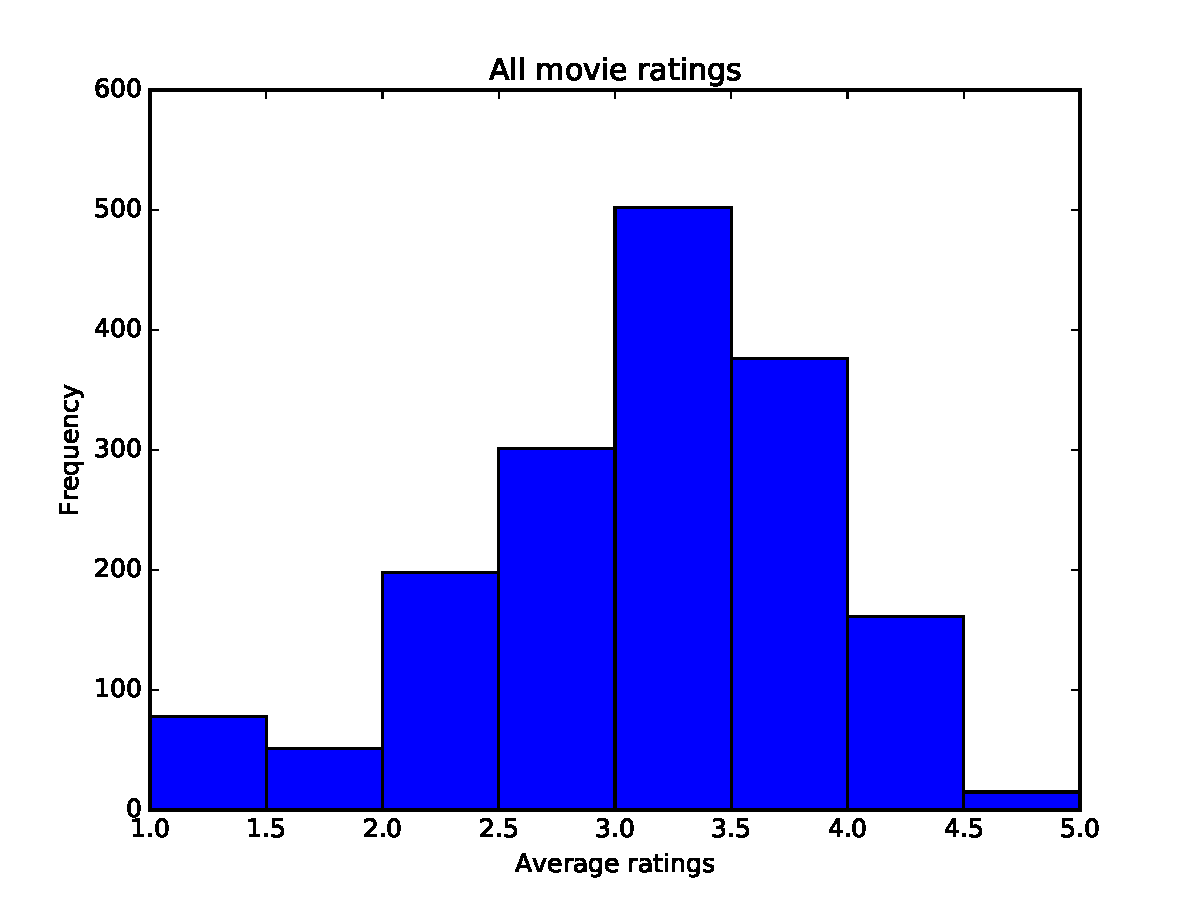
\includegraphics[width=\textwidth]{all_movie_ratings}
	\caption{Average ratings for all movies in MovieLens.} \label{fig:all-movie}
\end{figure}


Figure \ref{fig:all-movie-sorted} provides another view of the average ratings for all movie in the MovieLens dataset. We can observe that when the average ratings are integers, there are small numbers of ratings, indicating that the average ratings at those integer values may not be reliable.

\begin{figure}[H]
	\centering
	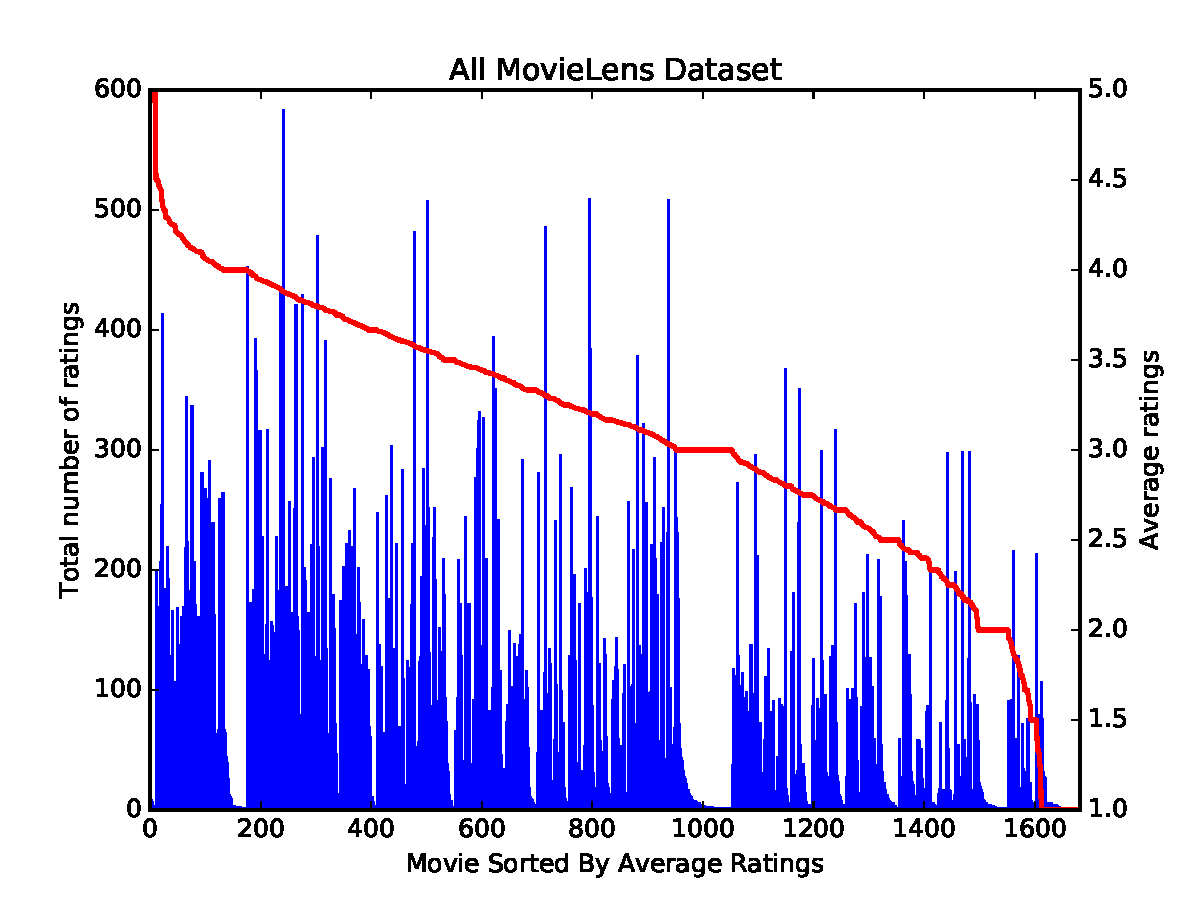
\includegraphics[width=\textwidth]{sorted_ratings}
	\caption{Average ratings for all movies in MovieLens sorted according to the average ratings. Red line represents the average ratings, and blue bars represent the total number of ratings.} \label{fig:all-movie-sorted} 
\end{figure}

Figures \ref{fig:top-10-best} and \ref{fig:top-10-popular} show distribution of ratings for the top 10 best movies and top 10 most popular movies respectively. First, we can see that the top 10 best movies have small numbers of ratings, but they are all 5 resulting in average ratings of 5. This observation indicates that the ratings are not too reliable. Second, the top most popular movies tend to have high ratings. This observation indicates that a popular movie tends to be a good movie. It might also indicate that a good movie tends to be a popular movie. The causality is unclear, but good movies seem to be correlated to popular movies, making logical sense. 

\begin{figure}[H]
	\centering
	\subfloat[Top 10 best movies] {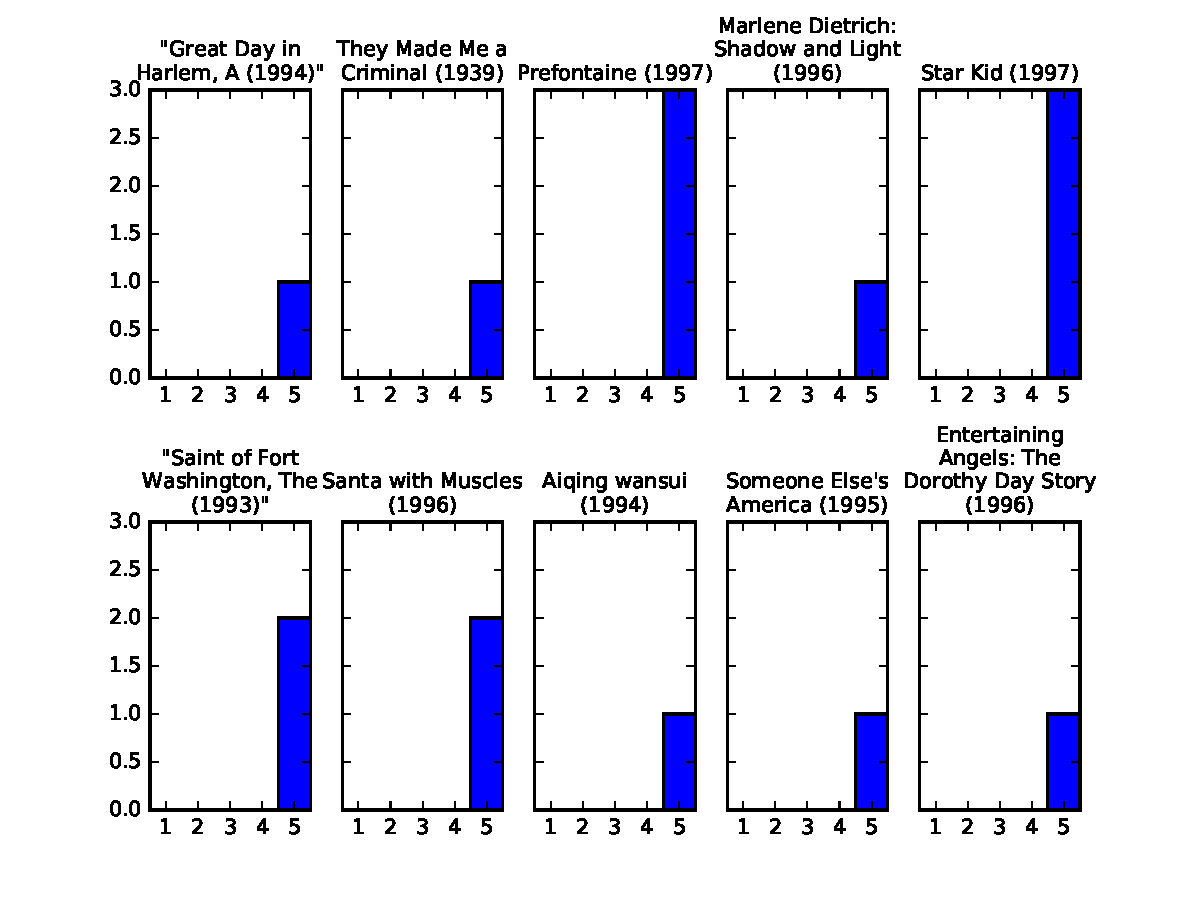
\includegraphics[width=0.8\textwidth, trim = 0cm 0mm 0cm 1cm, clip=true] {top_10_best_movie}\label{fig:top-10-best}}\\
	\subfloat[Top 10 most popular movies] {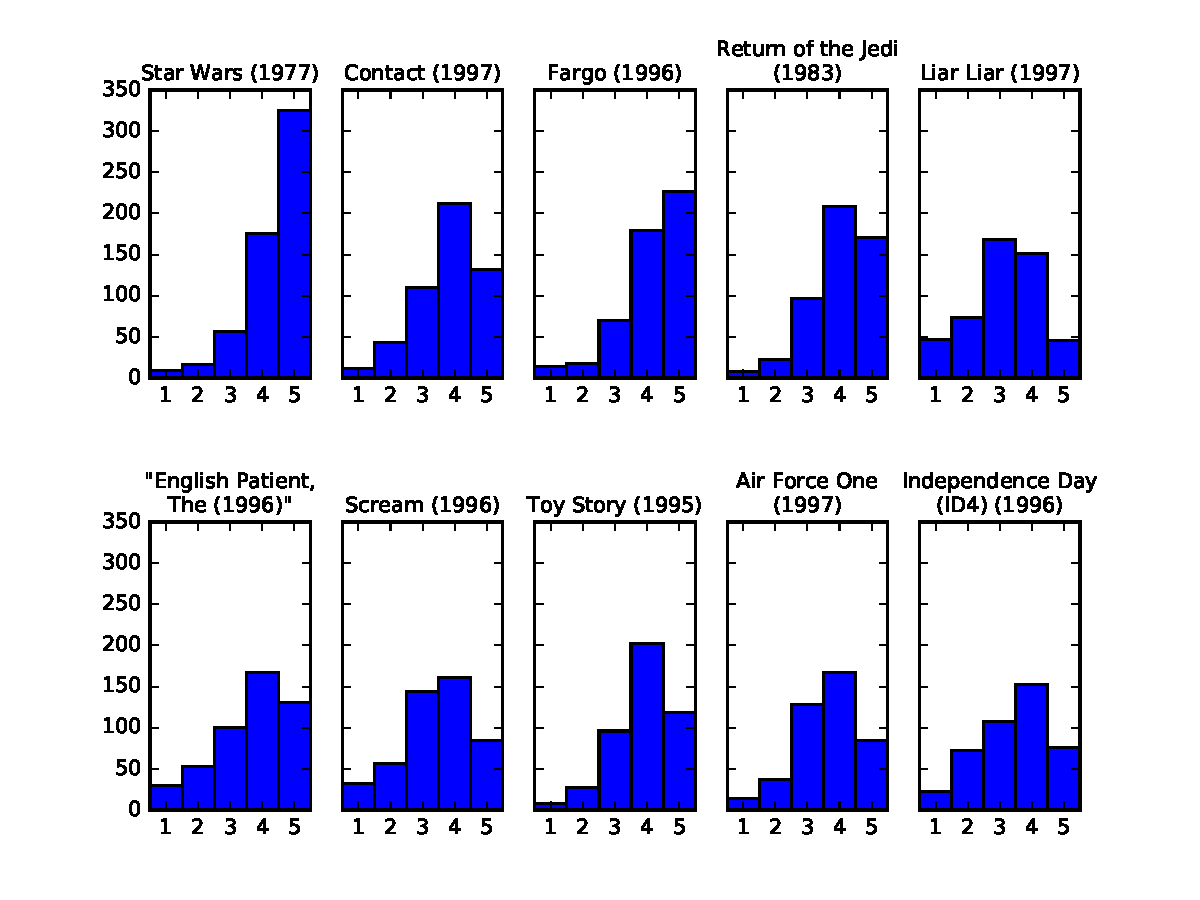
\includegraphics[width=0.8\textwidth, trim = 0cm 0mm 0cm 1.3cm, clip=true]{top_10_popular_movie}\label{fig:top-10-popular}}
	\caption{Ratings of top movies.} 
\end{figure}

Figure \ref{fig:average-3-genres} shows the average ratings of all movies in four different genres -- children, fantasy, horror, and documentary. There are fewer fantasy movies than children, horror, and documentary. The first three genres seem to have average ratings of about 2.5 to 3. The documentary genre has more high average ratings than the rest. In fact, the documentary genre seems to have more movies with above average ratings than movies with below average ratings. The other genres are more balanced. The documentary movies have a peak near average ratings of 3 to 3.5 and a small peak near average ratings of 1 to 1.5. This result indicates that documentaries are either really bad or good (above average ratings of 3).


\begin{figure}[H]
	\centering
	\subfloat[Children]{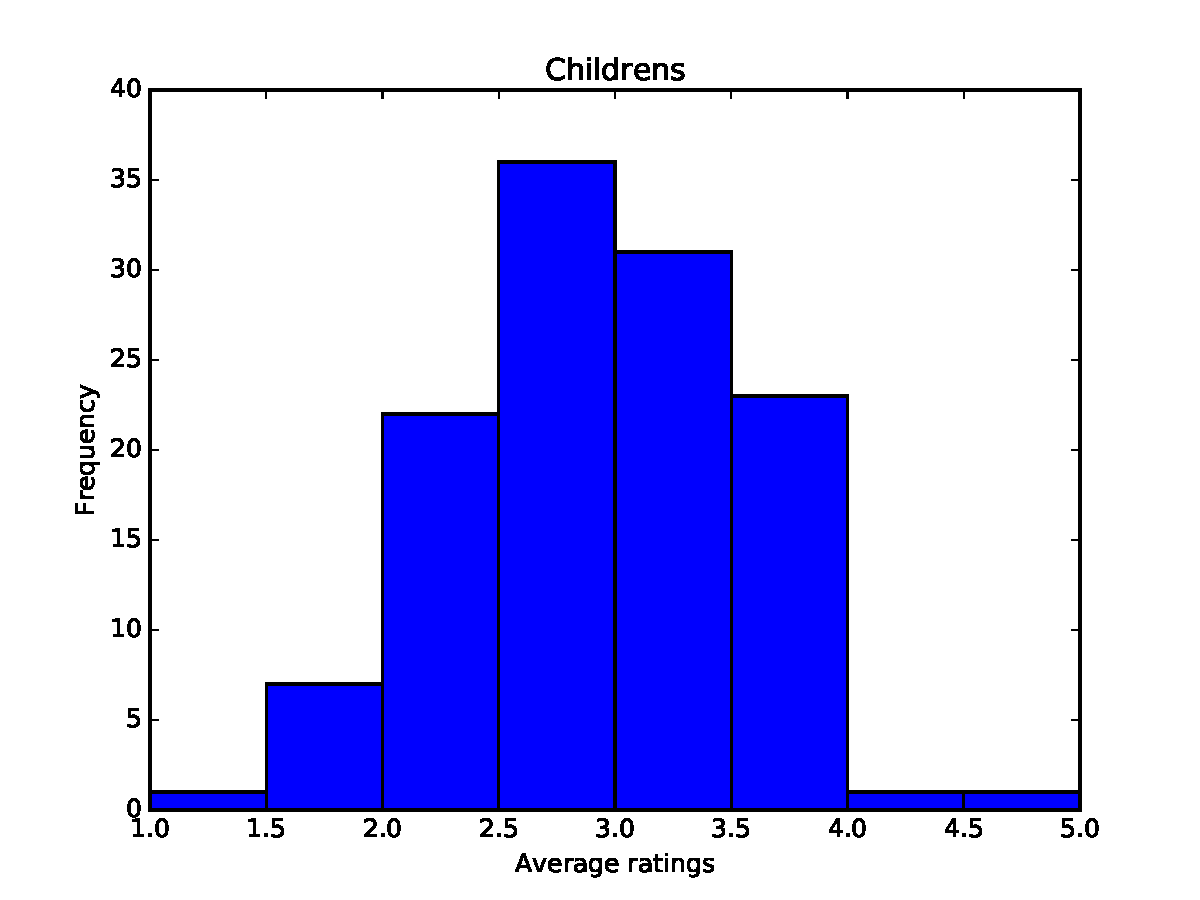
\includegraphics[width=0.45\textwidth, trim = 1cm 0mm 2cm 0mm, clip=true]{movie_genre_4}}
	\subfloat[Fantasy]{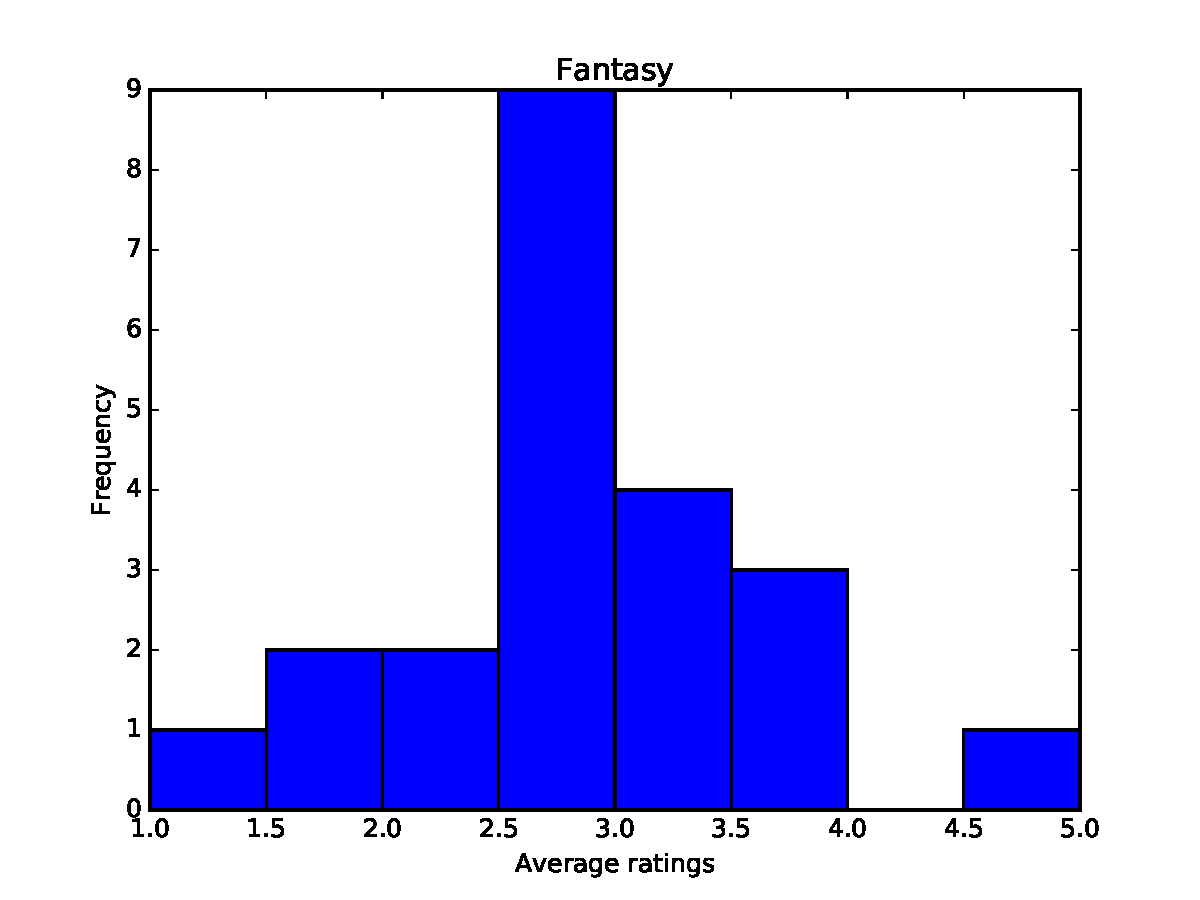
\includegraphics[width=0.45\textwidth, trim = 1cm 0mm 2cm 0mm, clip=true]{movie_genre_9}}\\
	\subfloat[Horror]{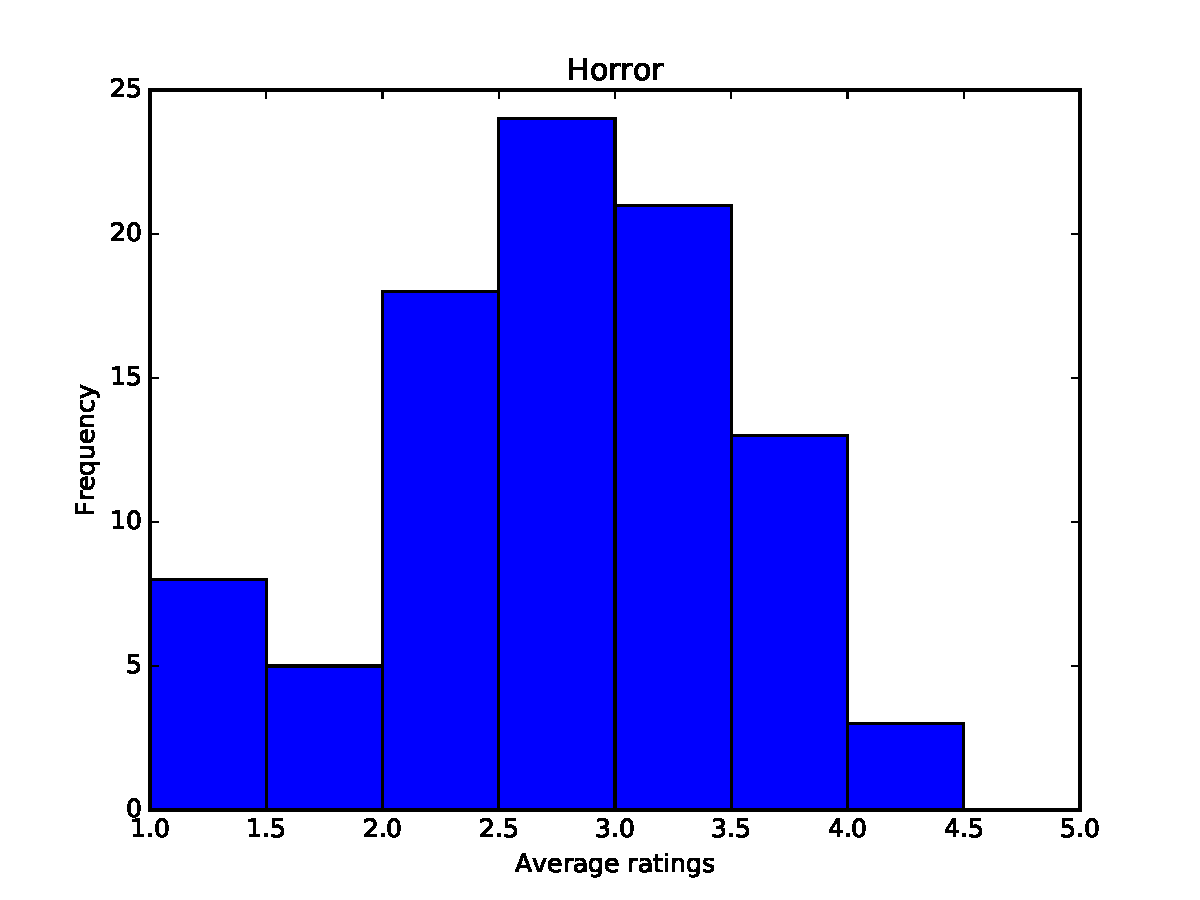
\includegraphics[width=0.45\textwidth, trim = 1cm 0mm 2cm 0mm, clip=true]{movie_genre_11}}
	\subfloat[Documentary]{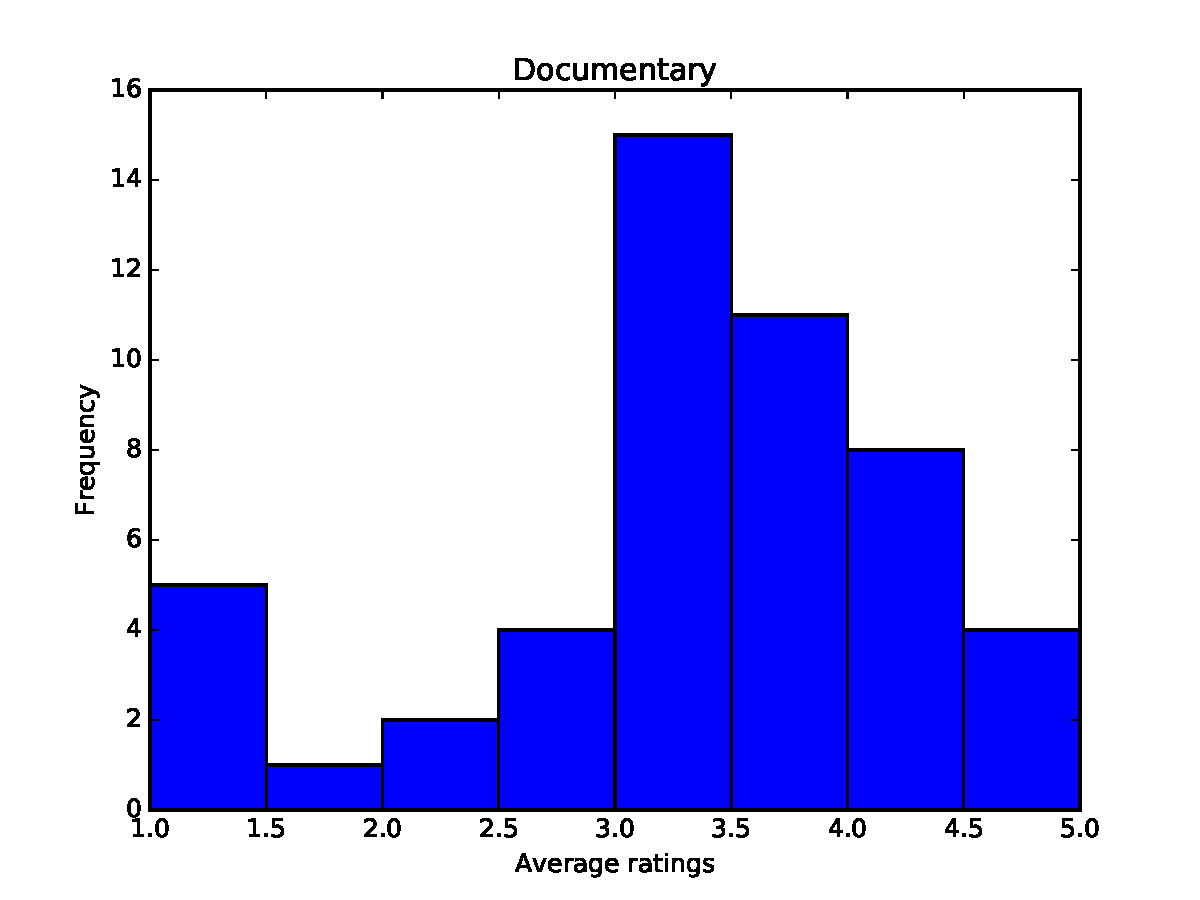
\includegraphics[width=0.45\textwidth, trim = 1cm 0mm 2cm 0mm, clip=true]{movie_genre_7}}
	\caption{Average ratings of all movies in four different genres.} \label{fig:average-3-genres}
\end{figure}
